\documentclass[a4paper,11pt]{article}

\usepackage[francais]{babel}
\usepackage[utf8]{inputenc}
\usepackage[official]{eurosym}
\usepackage{hyperref}
\usepackage{graphicx}
\usepackage{float}
\usepackage{amsmath,amsfonts,amssymb,amsthm}
\usepackage{algorithmic, algorithm}

\begin{document}
\hskip-2.7cm
  \begin{minipage}[c]{17cm}
  \vskip-2cm
    \begin{minipage}[c]{2cm}
      
\includegraphics[width=2cm]{img/logo-telecom-paristech.png}
    \end{minipage}
    \begin{center}
      \vspace*{2cm}

      {\LARGE Project Report}

      {\LARGE \textbf{Turing's Morphogenesis}}

      \vspace*{1cm}

      {\large \textbf{Olivier Le Floch},} code written with Thomas Deniau,
      March 20, 2009
    \end{center}
  \end{minipage}

\section{Introduction}

The phenotypes of multicellular living organisms such as mammals exhibit many
specific and complex shapes and textures. Since they have a rather limited
number of genes -- about 20.000 for humans \cite{human_genome} -- the
mechanics that generate these shapes must be very simple. In particular, this
means that they very probably use a limited number of chemicals that interact
together in a chaotic manner to form emergent complex patterns. In 1952,
Turing \cite{turing} proposed a simple diffusion-reaction model to try to
account for the observed genesis of planar patterns with only two chemicals :
$A$ is a pigmented catalytic molecule, and $B$ destroys $A$. The creation of
$B$ and $A$ is catalyzed by $A$. Additionally, both $A$ and $B$ follow a
standard diffusion differential equation. Our program solved the following
differential equation system based on Turk's \cite{turk} work on texture
generation :

\begin{eqnarray}
  A(t) &=& F(A, B) + D_A \nabla^2 A \\
  B(t) &=& G(A, B) + D_B \nabla^2 B
\end{eqnarray}

where $F(A, B) = D_s (16 - A B)$ and $G(A, B) = A B - B - \beta$. $D_A$ and
$D_B$ are diffusion speeds for both chemicals, $D_S$ is the reaction speed,
and $\beta$ is the decay rate of $B$.

\section{Technical solutions and challenges}

As can be seen in the \verb|README| file for \verb|PyMoprhogenesis|, we
implemented this solution in a graphical application based on Qt and OpenGL
using python bindings. The application can also be launched from the command
line in order to be able to easily specify parameters for automated batch
runs.

We encountered two problems in implementing this project : poor performance
for mathematical calculations in python, and sensitivity of the output to
small changes in the input parameters ($D_A$, $D_B$, $D_s$, $\beta$).

To improve performance, we used Blitz++ \cite{weave} \cite{performancepython}.
This allowed us to manipulate NumPy arrays in python when speed wasn't an
issue, i.e. for glue code : passing the image to OpenGL as a texture was coded
purely in python, for instance. On the other hand, when performance was
required, for instance for the diffusion calculations, we were able to
seamlessly manipulate the same arrays in C++ code directly embedded in our
python code, and compiled and cached at run-time so as to have no explicit
compilation phase and near-native performance. We didn't do any rigourous
benchmarks, but the performance improvement was by several orders of
magnitude, going from more than a second per iteration to less than a
hundredth of a second.

To find adequate values for the parameters, we added an option to
automatically run the program from a set of given parameter values, and coded
a script that outputted 80 images obtained from these values at iteration
1000. We then compared the images, and be exploring values around the most
interesting image outputs, obtained some results summed up in section
\ref{sec:results}.

\section{Results} % (fold)
\label{sec:results}

Our goal was to produce textures that were as close as possible to real world
animal skin patterns. As we were using only one pigmented chemical, and since
the parameter space is very large, the results we obtained were not perfect.
We did however obtain the following series of pictures, with accompanying
parameter ranges.

\subsection{Stripes} % (fold)
\label{sub:stripes}

We obtained stripes with $D_a > 10 * D_b$. The width of the stripes decreases when $D_s$ increases.

\begin{figure}[!ht]
  \centering
  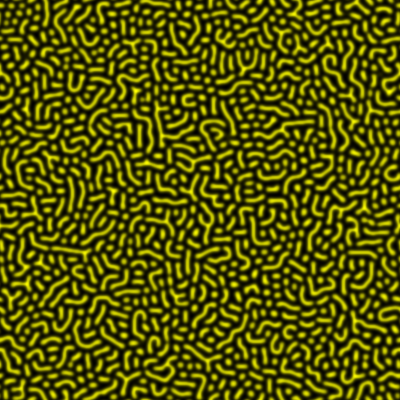
\includegraphics[width=5cm]{img/stripes.png}
\end{figure}

% subsection stripes (end)

\subsection{Dots} % (fold)
\label{sub:dots}

We obtained dots with $5 * D_b > D_a > 3 * D_b$. The contrast of the dots
relative to the background decreases when $D_s$ increases.

\begin{figure}[!ht]
  \centering
  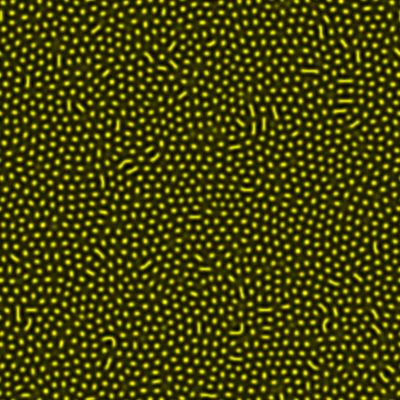
\includegraphics[width=5cm]{img/dots.png}
\end{figure}

% subsection dots (end)

\subsection{Spots} % (fold)
\label{sub:spots}

We obtained relatively large spots with $D_a >> D_b$. The spots' intensity decreases when $D_s$ increases.

\begin{figure}[!ht]
  \centering
  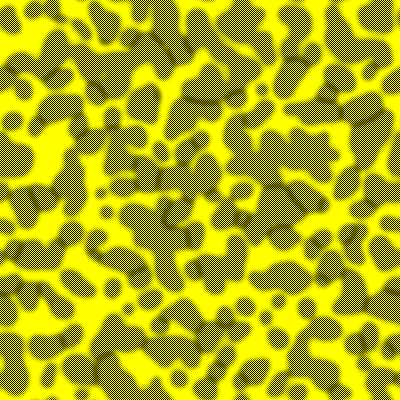
\includegraphics[width=5cm]{img/spots.png}
\end{figure}

% subsection dots (end)

% section results (end)

\section{Future work}

This work can be improved in the future by using machine learning algorithm
trained on local shape and texture features, extracted using wavelet
approaches for instance, to search more efficiently for interesting values of
the input parameters.

Additionally, as not all textures seem to be reachable through this model when
starting with a purely random, white-noise, isotropic initial distribution for
both chemicals, we may need to add an anisotropic initialisation to allow us
to generate more zebra like, strongly anisotropic textures.

\section{Conclusion}

In conclusion, we produced a python program reproducing results that show that
very simple chemical reactions can account for the creation of shape in living
beings. Our program also provides an interesting technological overview of
simple to deploy technologies to quickly develop applications in python with
performance sufficient for time-consuming numerical calculations.

\begin{thebibliography}{99} % (fold)

\bibitem{turing}
  Alan Turing,
  The Chemical Basis of Morphogenesis,
  \emph{Transactions of the Royal Society B}, Vol. 237, pp. 37-72 (August 14, 1952).

\bibitem{turk}
  Greg Turk,
  Generating Textures on Arbitrary Surfaces Using Reaction-Diffusion,
  \emph{Computer Graphics}, Vol. 25, No. 4, (SIGGRAPH 91), pp. 289-298, July 1991.

\bibitem{human_genome}
  International Human Genome Sequencing Consortium,
  Finishing the euchromatic sequence of the human genome.
  \emph{Nature}, 431 (7011): 931-45, 2004.

\bibitem{lawlor}
  Orion Sky Lawlor,
  Reaction-Diffusion Textures, \\
  \url{http://charm.cs.uiuc.edu/users/olawlor/projects/2003/rd/}

\bibitem{jennings}
  Christopher G. Jennings, \\
  Turing's Reaction-Diffusion Model of Morphogenesis, \\
  \url{http://www.sfu.ca/~cjenning/toybox/turingmorph/}

\bibitem{performancepython}
	Prabhu Ramachandran et al.,
  A comparison of weave with NumPy, Pyrex, Psyco, Fortran and C++ for solving Laplace's equation, \\
	\url{http://www.scipy.org/PerformancePython}

\bibitem{weave}
	Weave, a python package allowing the inclusion of C/C++ code within python code,
	\url{http://www.scipy.org/Weave}

\end{thebibliography}% (end)

\end{document}
